\DiaryEntry{Triangular Numbers}{2015-10-08}{Maths}

\subsection{Basics}

Based upon \href{https://en.wikipedia.org/wiki/Triangular_number}{Wikipedia}.

These are the number of nodes that form an equilateral triangle, as
shown below.

\todo{FIGURE}
\begin{figure}
\centering
%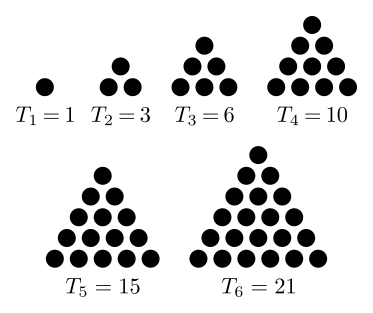
\includegraphics{/images/triangular_numbers.svg}
\end{figure}

The $n$-th triangle number is the number of nodes composing a triangle with n nodes on a side, and is equal to the sum of the $n$ natural numbers from
$1$ to $n$. That is,

\[ T_n = \sum_{i=0}^n n = \frac{n(n+1)}{2} \]

We had this sum before but there are two other alternatives; one based on an geometric argument; the other uses generating functions.

\subsubsection{Geometric Argument}

Consider the Figure below; there are $5 \times 5 = 25$ nodes. The green and black ones are each $T_4$, and there are
$5$ red ones. Therefore, the total number of nodes can also be expressed as $2 \times T_4 + 5$.

\todo{FIGURE}
\begin{figure}
\centering
%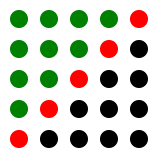
\includegraphics{/images/triangular_numbers_2.svg}
\end{figure}

Generalizing to arbitrary $n$, we have

\[n^2 = 2 \times T_{n-1} + n \rightarrow T_{n-1} = \frac{n^2 - n}{2} = \frac{n(n-1)}{2} \]

or

\[T_{n} = \frac{n(n+1)}{2}\]

This is a classic of counting the same arrangements in a different
(preferably simpler) way.

\subsubsection{Generating Functions}

Converting the sum $T_n \sum_{i=0}^n i$ into a recurrence relation, we obtain $T_n = T_{n-1} + n$; or equivalently

\[ T_{n+1} = T_n + (n+1); \qquad T_0 = 0\]

We can convert this into an expression for the generating function
$A(z)$ of $T_n$; namely

\[ \frac{A(z)-T_0}{z} = A(z) + \sum_{n \geq 0}n z^n + \sum_{n \geq 0} z^n \]

For the expression $\sum_{n \geq 0}n z^n$ we do the following: Consider the all-one series which generating function is $B(z) = \sum_{n \geq 0} 1 z^n = \frac{1}{1-z}$. We seek $n z^n$; this corresponds to $z B(z) = \frac{z}{(1-z)^2}$.

We therefore have

\[ \frac{A(z)-T_0}{z} = A(z) + \frac{z}{(1-z)^2} + \frac{1}{1-z} \rightarrow A(z) = \frac{z}{(1-z)^3}\]

A series expansion yields

\begin{verbatim}
      2     3      4      5      6      7      8      9
x + 3x  + 6x  + 10x  + 15x  + 21x  + 28x  + 36x  + 45x  + ...
\end{verbatim}

Another way would be to consider the sequence $1,2,3,4,\ldots$ with the generating function $A(z) = \sum_{n \geq 0} n z^n = \frac{z}{(1-z)^2}$. We want to obtain the sequence of the partial sums; the corresponding generating function is $\frac{A(z)}{1-z} = \frac{z}{(1-z)^3}$.

\subsubsection{Other Characteristics}

From the definition of the $T_n$, we have the following property:

\[ T_n + T_{n-1} = \frac{n(n+1)}{2} + \frac{n(n-1)}{2}  = n^2\]

and

\[ T_{n} - T_{n-1} = \frac{n(n+1)}{2} - \frac{n(n-1)}{2}  = n \]

Therefore, we have

\[ T_n + T_{n-1} = (T_{n} - T_{n-1})^2 \]

\subsection{Number of Line Segments}

Related to the triangular numbers are the numbers $L_n$ of direct connections between the objects; for example see the Figure below. For $n=4$ (red lines), we have $L_4 = 18$. Every node contributes
$3$ connections; therefore we have $L_n = 3 T_{n-1}$.


\todo{FIGURE}
\begin{figure}
\centering
%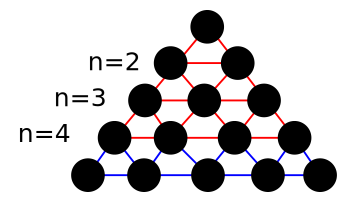
\includegraphics{/images/triangular_numbers_3.svg}
\end{figure}

A different argument leads to a recurrence relation for the $L_n$: If we have connections up to level $n$ ($n=4$) in the example above), then the next level adds another $3 \times n$ connections and we therefore have

\[ L_{n+1} = L_n + 3n\]

I.e. $L_5 = L_4 + 3 \times 4 = 18 + 12 = 30$.

\subsubsection{Generating Functions}

Just for the fun of it; we have

\[ \frac{A(z)}{z} = A(z) + 3 \sum_{n \geq 0} n z^n = A(z) + \frac{3z}{(1-z)^2} \rightarrow A(z) = \frac{3z^2}{(1-z)^3}\]

A series expansion yields

\begin{verbatim}
  2     3      4      5      6      7      8       9
3x  + 9x  + 18x  + 30x  + 45x  + 63x  + 84x  + 108x + ...
\end{verbatim}
